\section{Parallel Strategy and Performance}

\subsection{Parallel Strategy}

When \enzo\ is run on a distrubuted platform, some of the data is
replicated to all processors, while some remains on a single processor.
A description of the entire hierarchy (the position and size of each grid, as well
some other meta data) is stored on each processor.  This enables each
grid to know what grids are near it in the hierarchy, regardless of
where the data is.  The actual Baryon data (density, velocity, energy,
and any chemistry data) and particle data are stored on only one
processor.  Storing the entire hierarchy on all processor does create
some overhead, but in practice this is not an issue until one reaches
the extremely large scale.
  The code handles load balancing 
on a level-by-level basis such that the workload on each level is 
distributed as uniformly as possible across all processors.  Spatial locality of 
grids is not forced during message passing, for maximum flexibility (though not
necessarily maximum efficiency).  
The MPI message passing library\footnote{http://www-unix.mcs.anl.gov/mpi/}
 is used to transfer data between processors.

The performance of \enzo\ has been extensively studied using the
software package LCAPerf.  More on LCAPerf can be found in section
\ref{sec.performance} 

%old text
%Every processor 
%keeps a description of the entire grid hierarchy at all times, so that 
%each processor knows where all grids are.  However, baryon and particle 
%data for a given grid only exists on a single processor.  See 
%Figure~\ref{fig.2.amrhierarchy} for a schematic example of this.  



\begin{figure}
\begin{center}
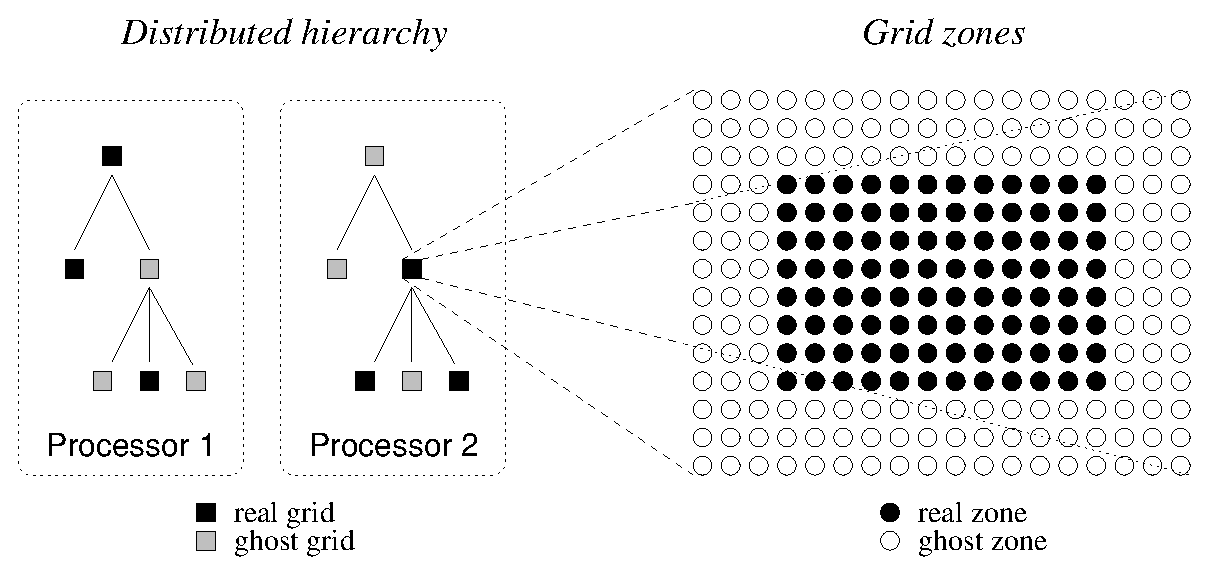
\includegraphics[width=0.4\textwidth]{figures/amr_hierarchy.eps}
\end{center}
\caption{\emph{Left:}  Example of a simple, distributed AMR hierarchy showing real and ghost grids.
\emph{Right:}  Example 2D \enzo\ grid showing real and ghost zones, as 
needed for the PPM hydro stencil. }
\label{fig:amr_hierarchy}
\end{figure}



% ----------------------------------

\subsection{Performance}
\label{sec.performance}

\red{
This is really James' section.  Profiling the code is very difficult because
of the many possible configurations that it can be run under.  In general,
we want to show both AMR and unigrid calculations scale, for cosmology runs
and for pure hydro (i.e. turbulence) runs.  The gravity scales far differently
than the hydro, so perhaps we should do a gravity-only (dark matter?) vs. 
hydro only (driven isothermal turbulence, non-gravitating) scaling?
We should also include performance information for some of the very large
simulations that we've done -- 2048$^3$ unigrid and 512$^3$ AMR runs.
}

\red{It seems like this section will be fiercely debated.  So have fun.}
